\Aufgabe{Datenfluss-Puzzle}{
    \begin{enumerate}
        \item Trefft euch mit der Gruppe, mit der ihr euer Datenflussdiagramm getauscht habt. Von eurer Lehrkraft bekommt ihr ausgedruckt die Lösungen für eure Einzeldiagramme und ein A3 Blatt als Untergrund.
        \item Fügt eure einzelnen Datenflussdiagramme zu einem Gesamtdiagramm zusammen. Nutzt hierfür ggf. eine Schere und fügt zusätzliche Datenflüsse und falls notwendig Funktionen ein.
        \item Überlegt euch:\\Welche Elemente kann man beim Zusammenfügen entfernen (ohne Information zu verlieren) und wieso?\\
            \LoesungLine{Datenblöcke zwischen 2 Funktionen (aber nur wenn Funktionsname aussagekräftig genug ist, um trotzdem zu verstehen, was gerechnet wird)}{3}
        \item Zeichnet \emphColB{nach dem gemeinsamen Vergleich mit der ganzen Klasse} ein möglichst stark vereinfachtes Gesamt-DFD zu Gruppe B auf die nächste Seite.
    \end{enumerate}

    \AttachVlg{\faFilePdfO}{_Aufgaben/resources/A06_Vlg.pdf}
}
    \ifbeamer
        \definesframe[false]{}{
            \centering
            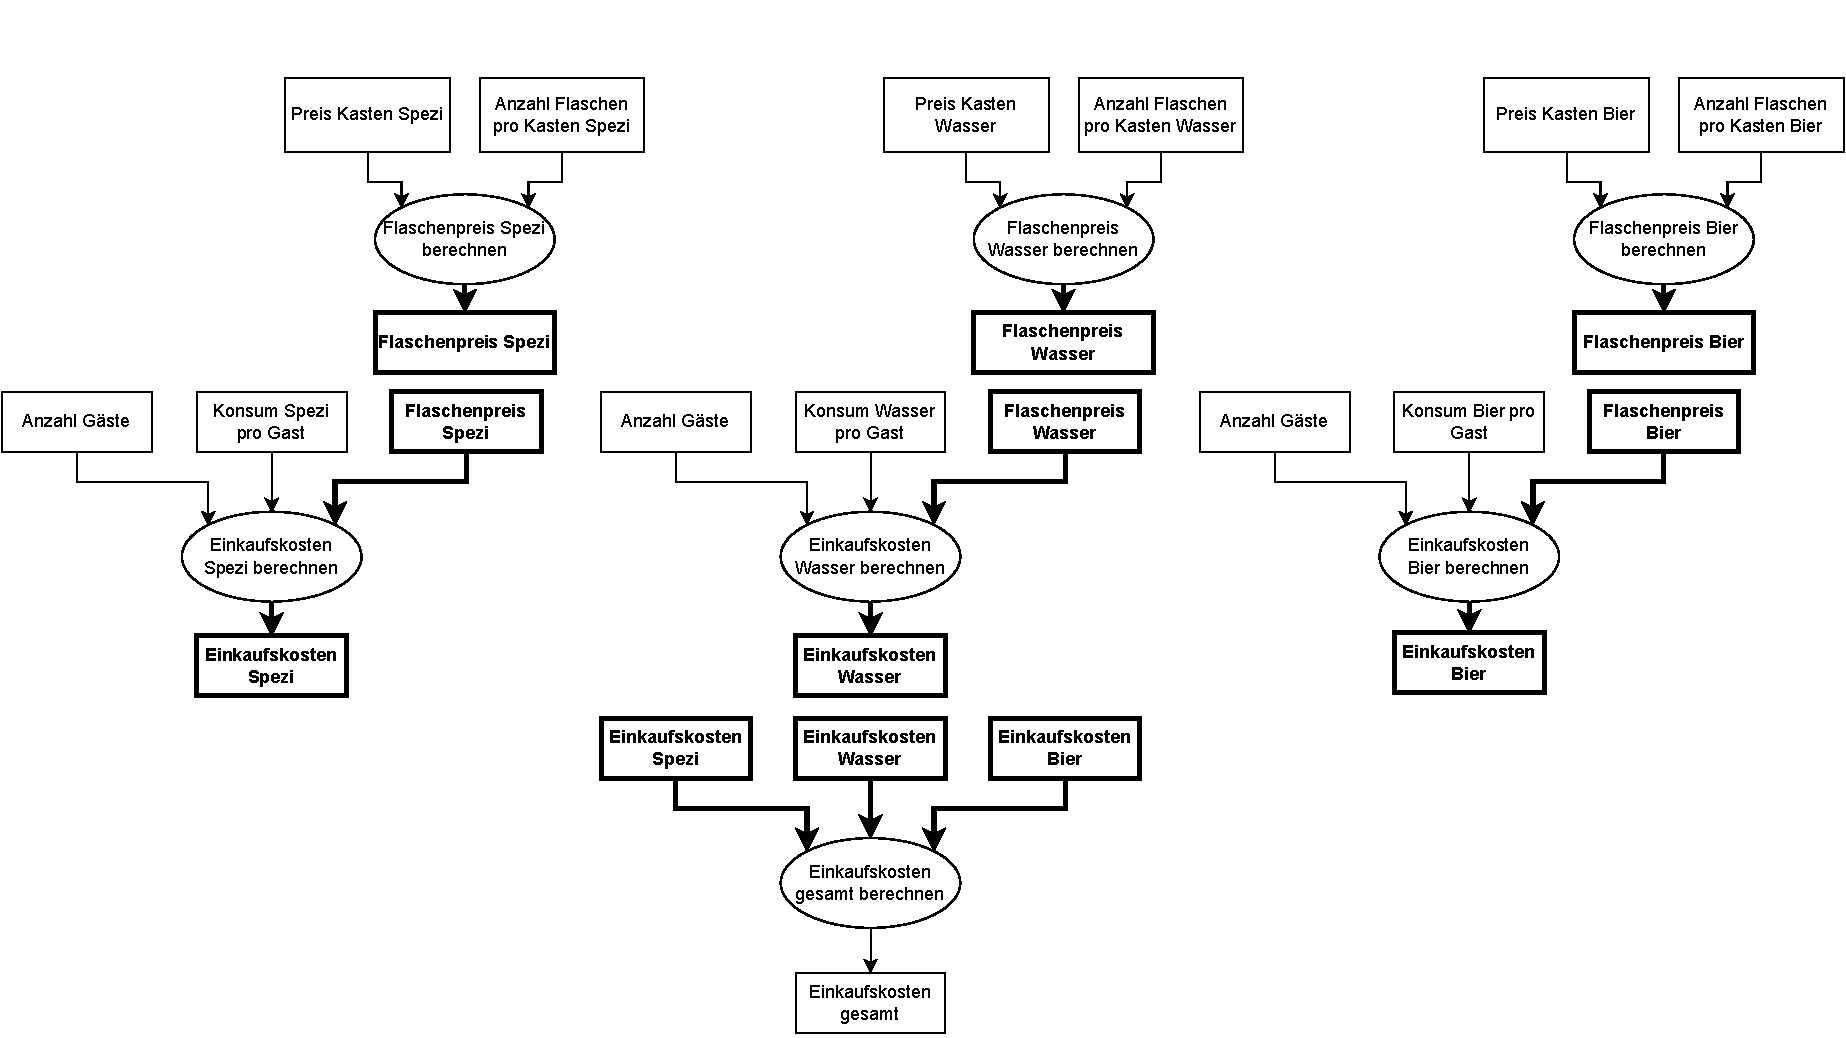
\includegraphics[width=\textwidth]{_Aufgaben/img/A06_Lsg_A01.pdf}
        }
        \definesframe[false]{}{
            \centering
            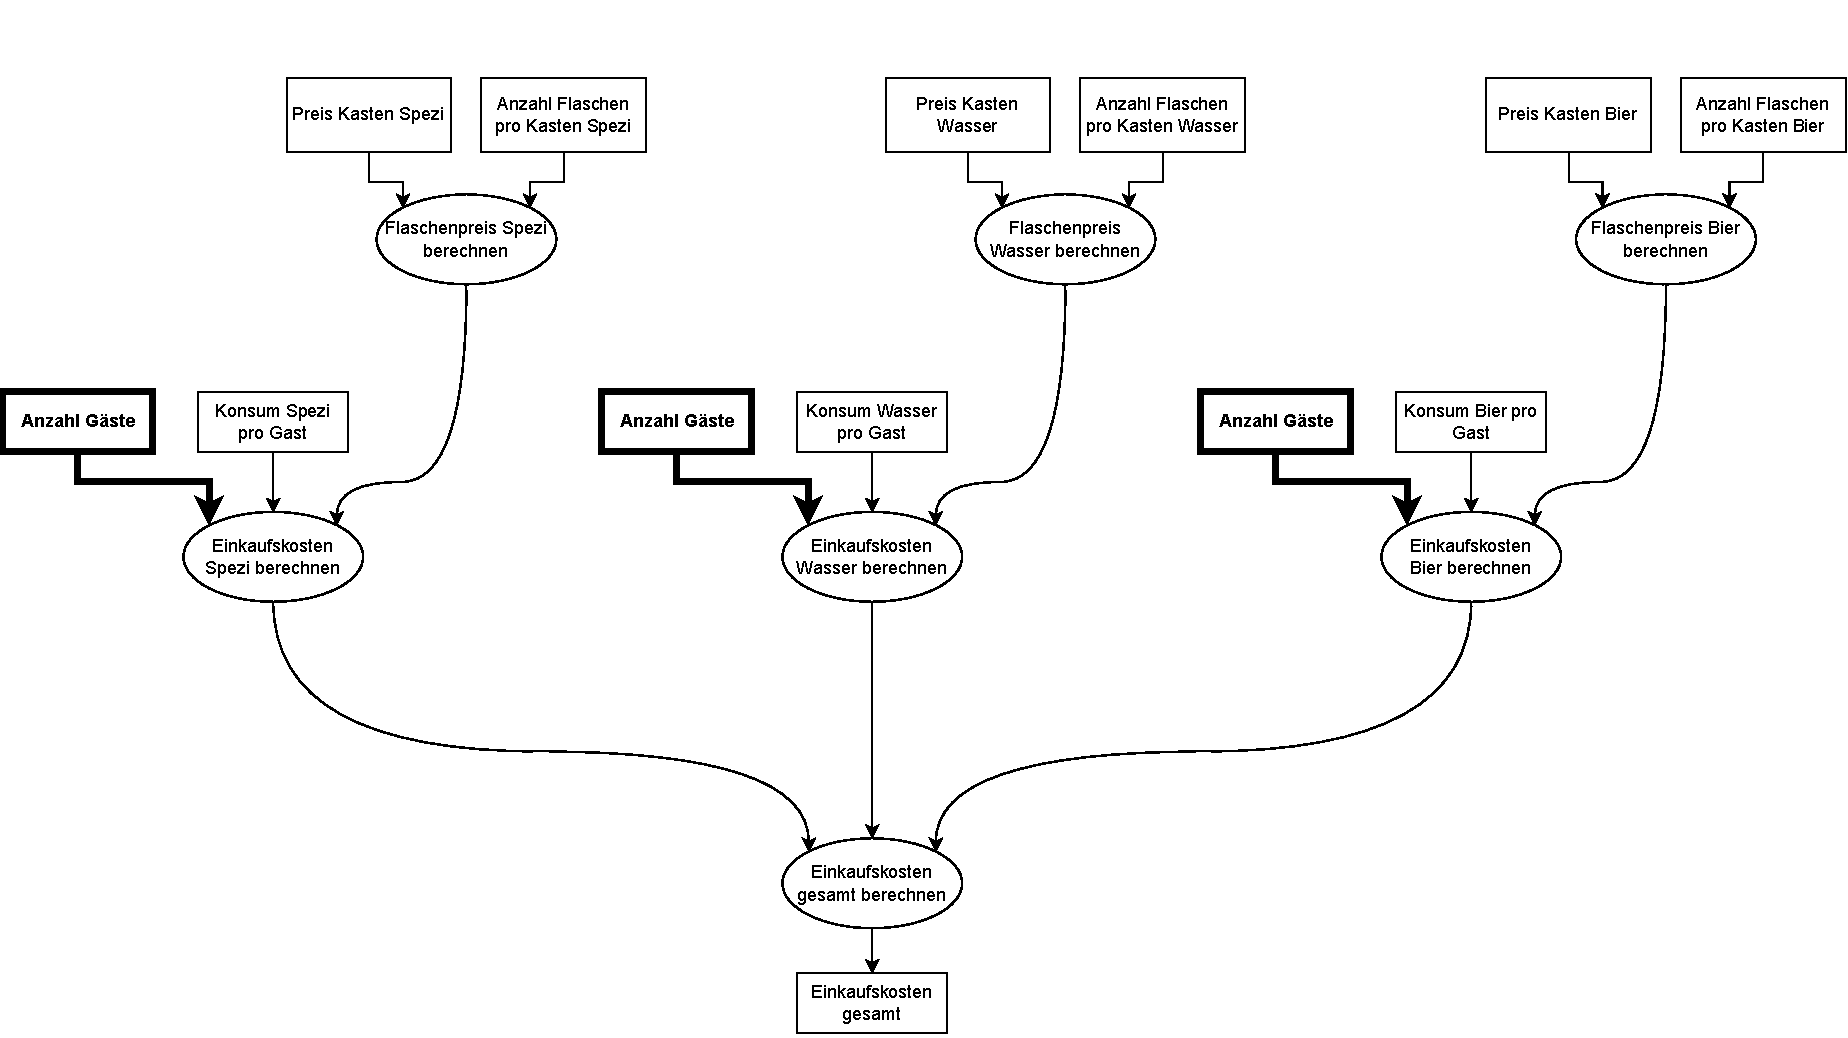
\includegraphics[width=\textwidth]{_Aufgaben/img/A06_Lsg_A02.pdf}
        }
        \definesframe[false]{}{
            \centering
            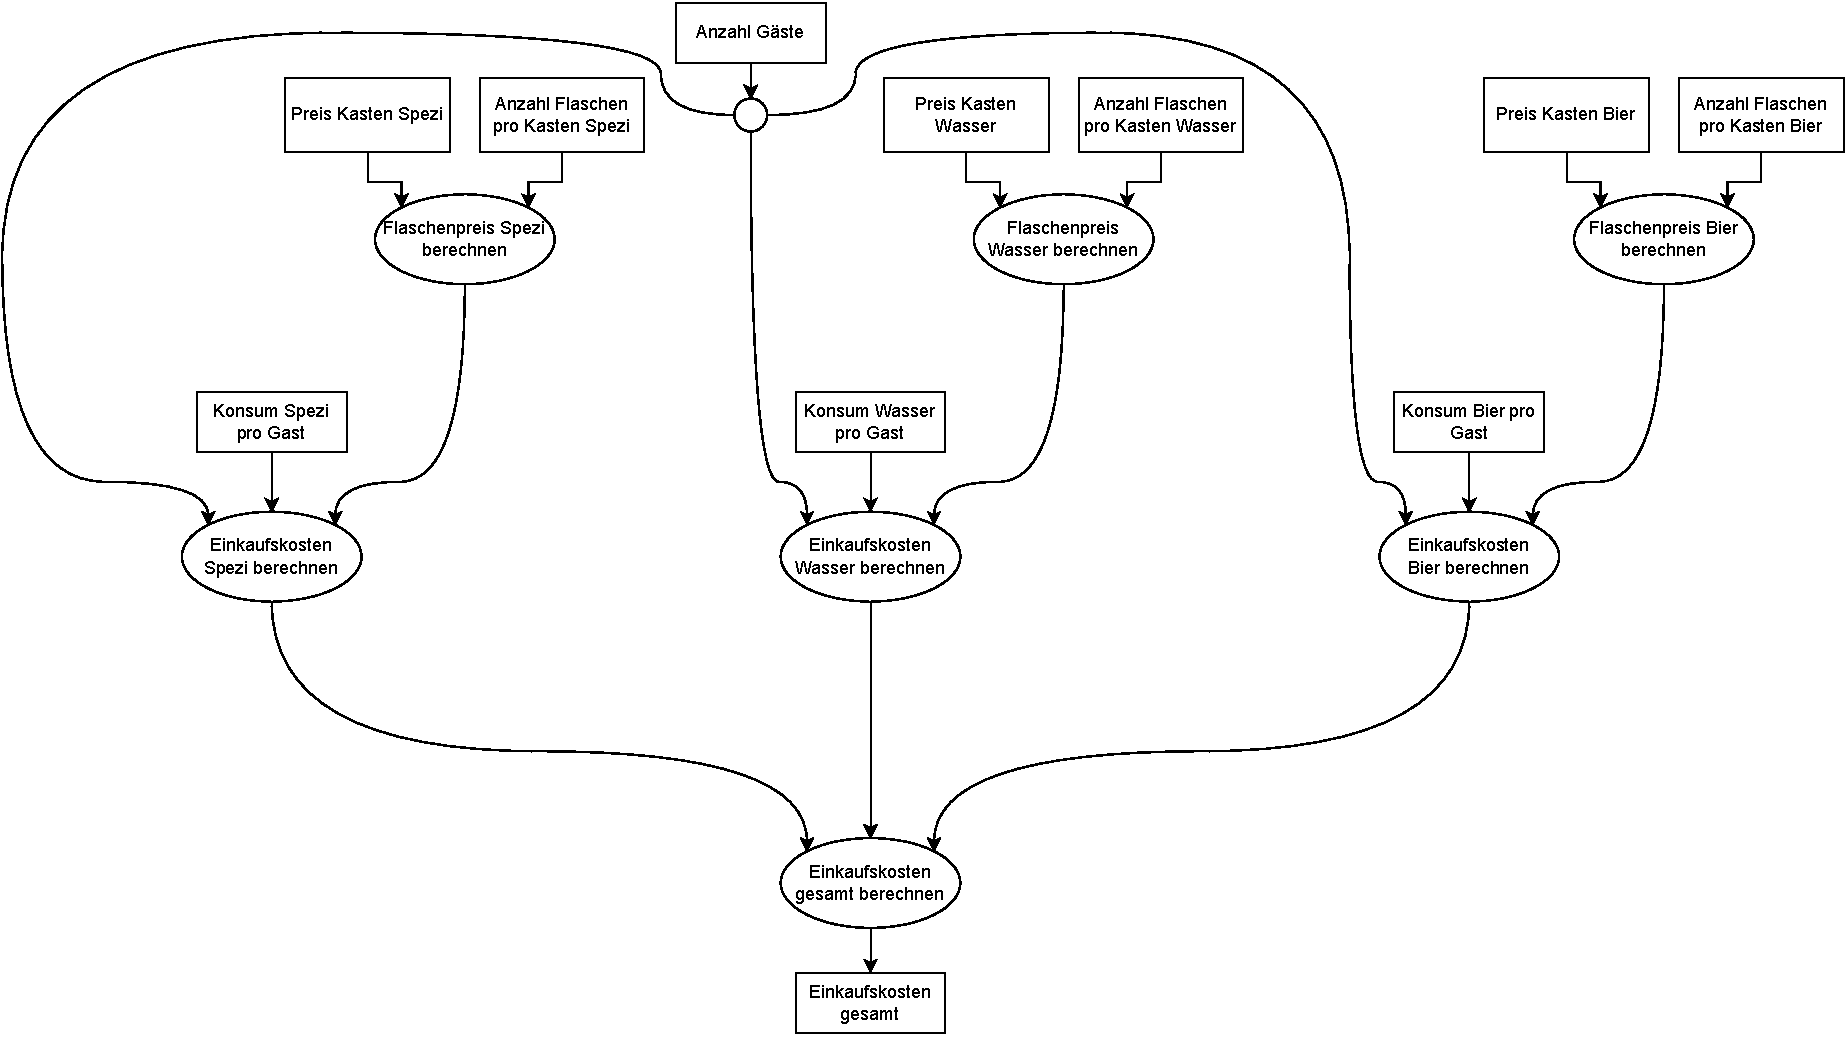
\includegraphics[width=\textwidth]{_Aufgaben/img/A06_Lsg_A03.pdf}
        }
    \else
        \UnterAufgabe{Gruppe A vereinfacht}{
            \Loesung{Gruppe A vereinfacht}
            
            \Loesung{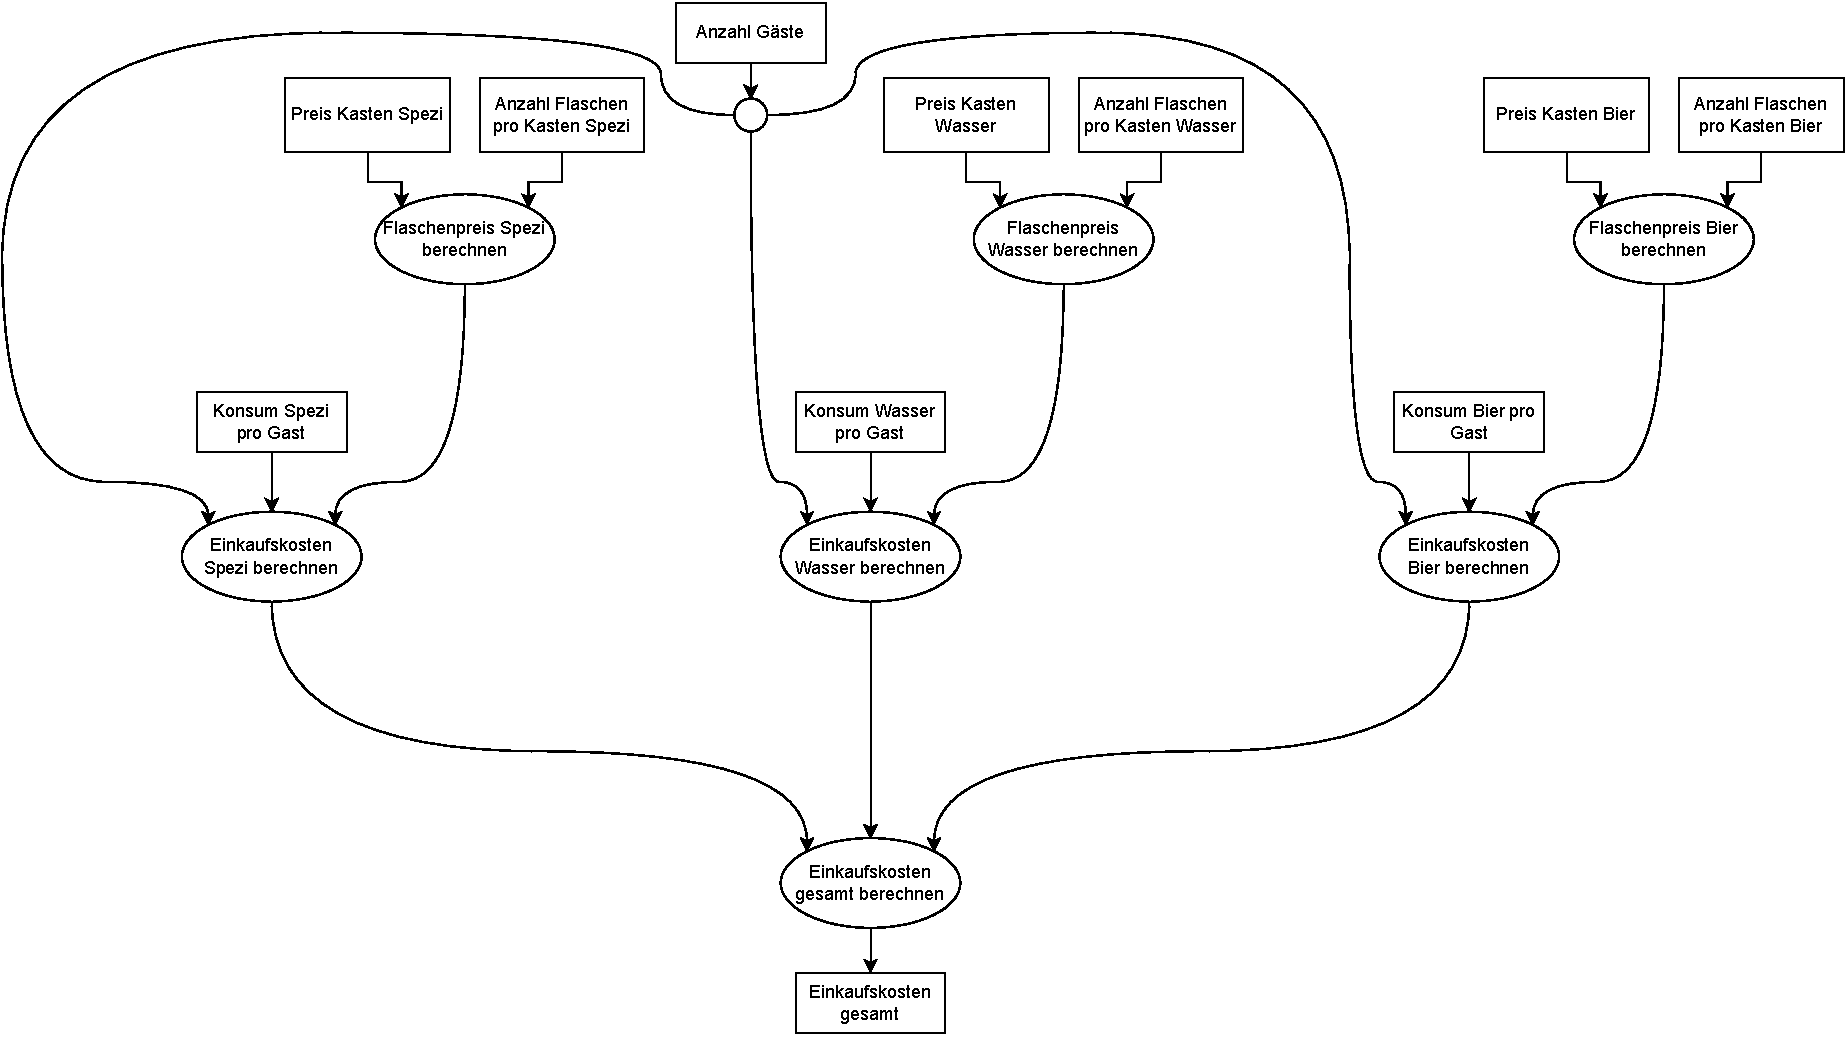
\includegraphics[width=\textwidth]{_Aufgaben/img/A06_Lsg_A03.pdf}}
        }
    \fi

    \ifbeamer
        \definesframe[false]{}{
            \centering
            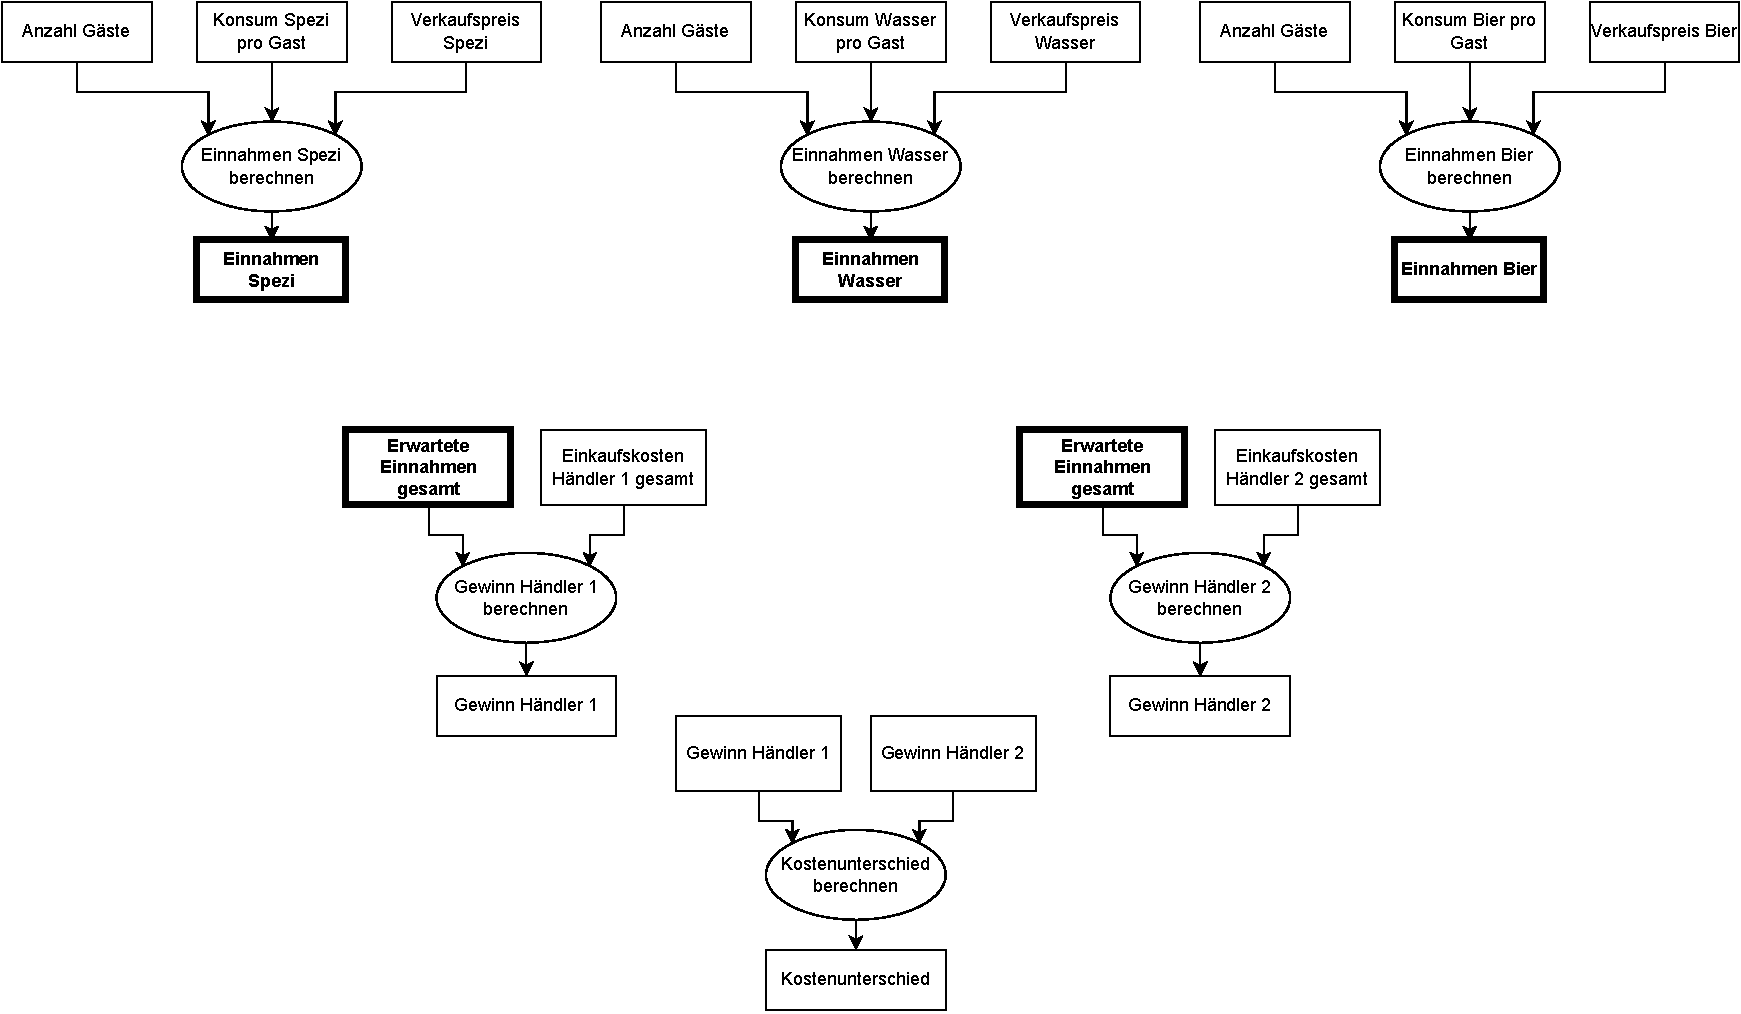
\includegraphics[height=\pageheight]{_Aufgaben/img/A06_Lsg_B01.pdf}
        }
        \definesframe[false]{}{
            \centering
            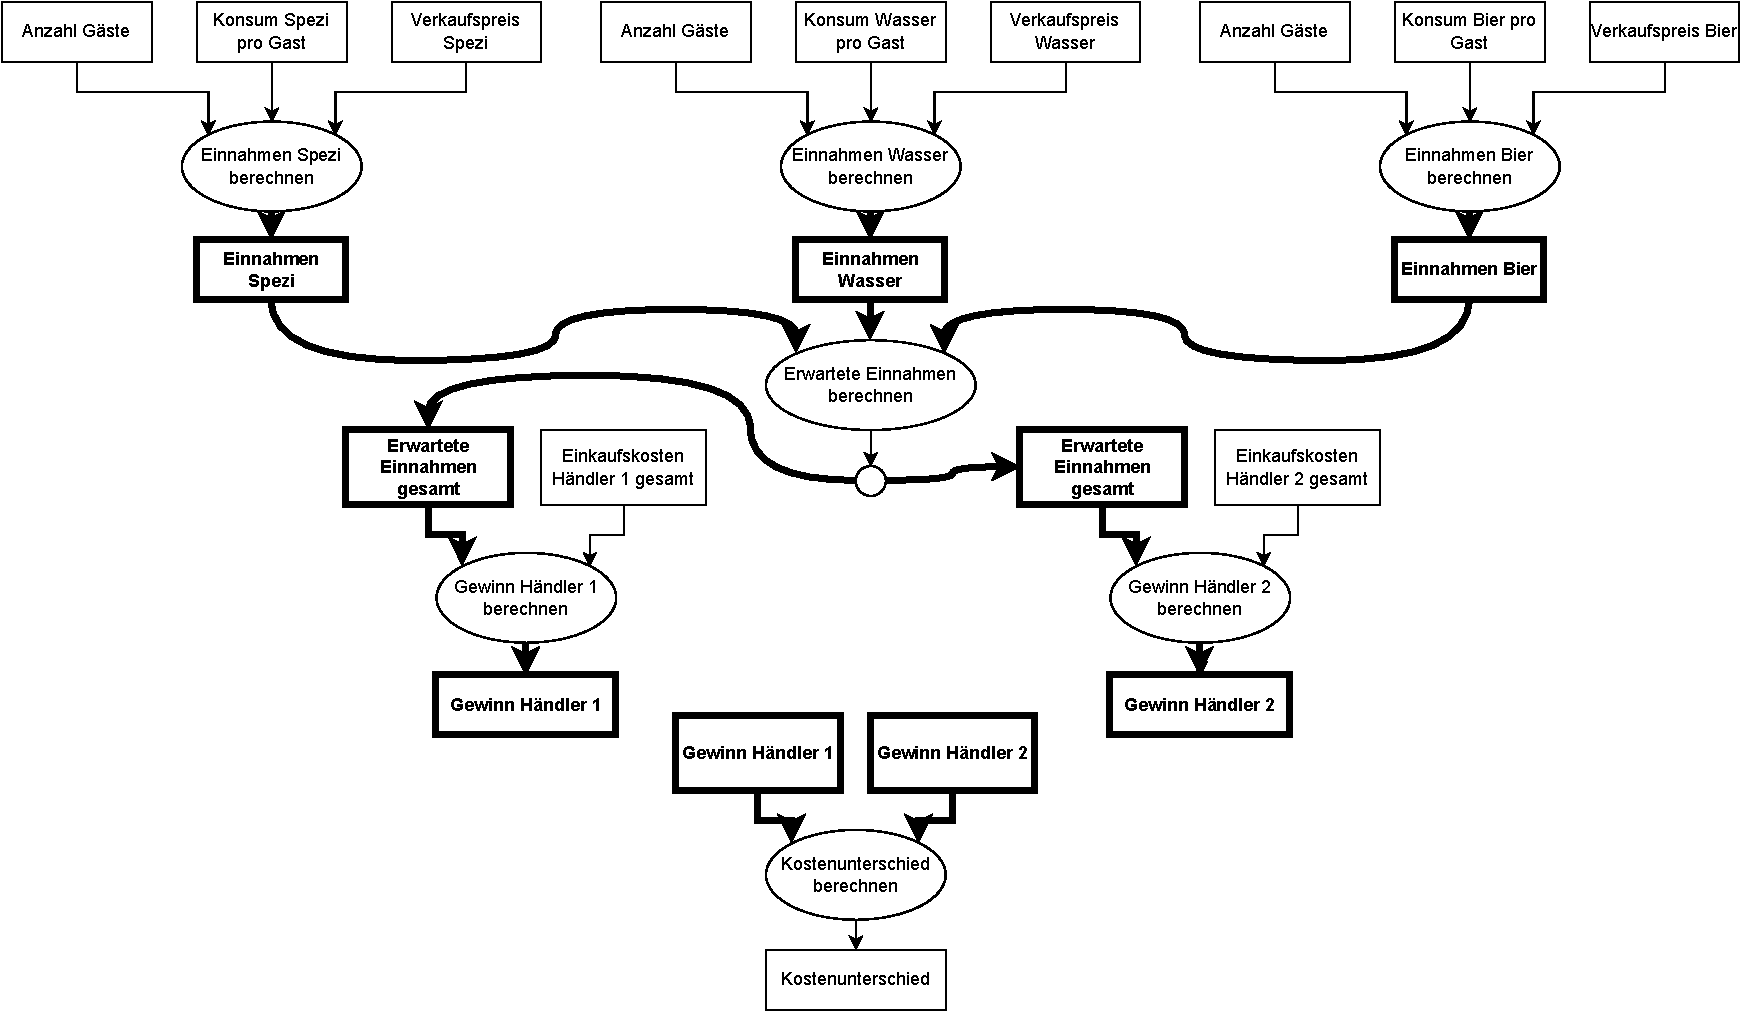
\includegraphics[height=\pageheight]{_Aufgaben/img/A06_Lsg_B02.pdf}
        }
        \definesframe[false]{}{
            \centering
            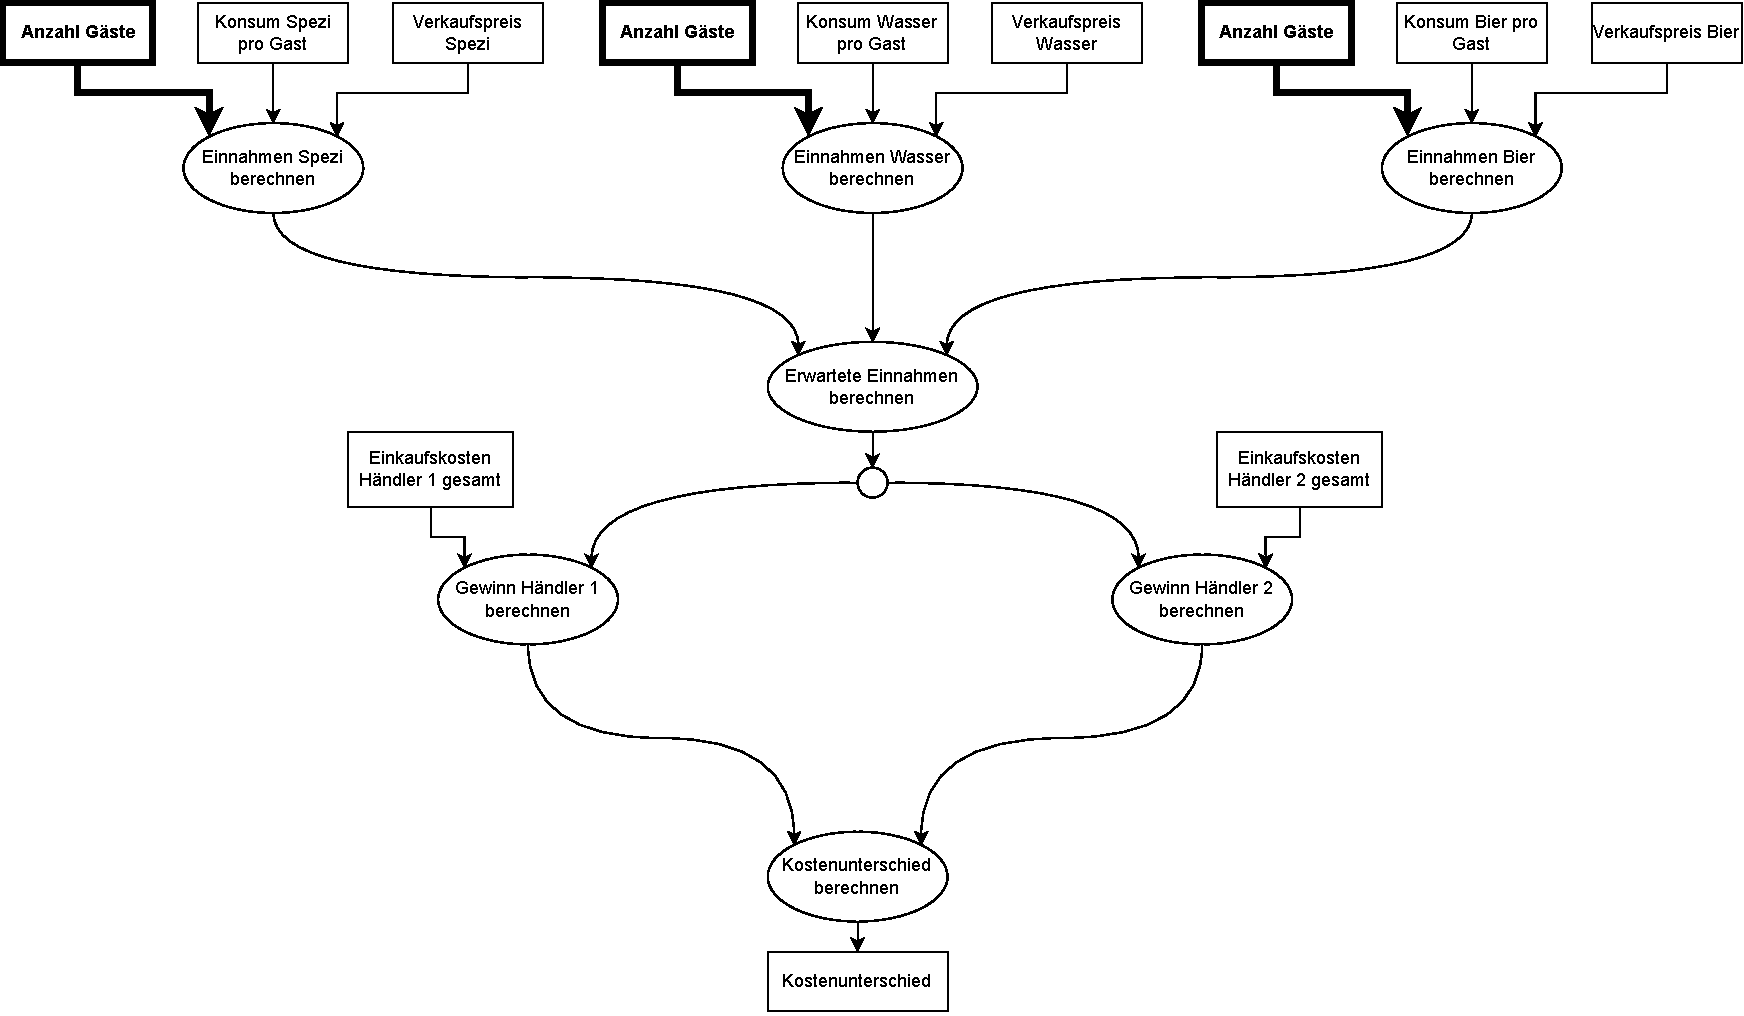
\includegraphics[height=\pageheight]{_Aufgaben/img/A06_Lsg_B03.pdf}
        }
        \definesframe[false]{}{
            \centering
            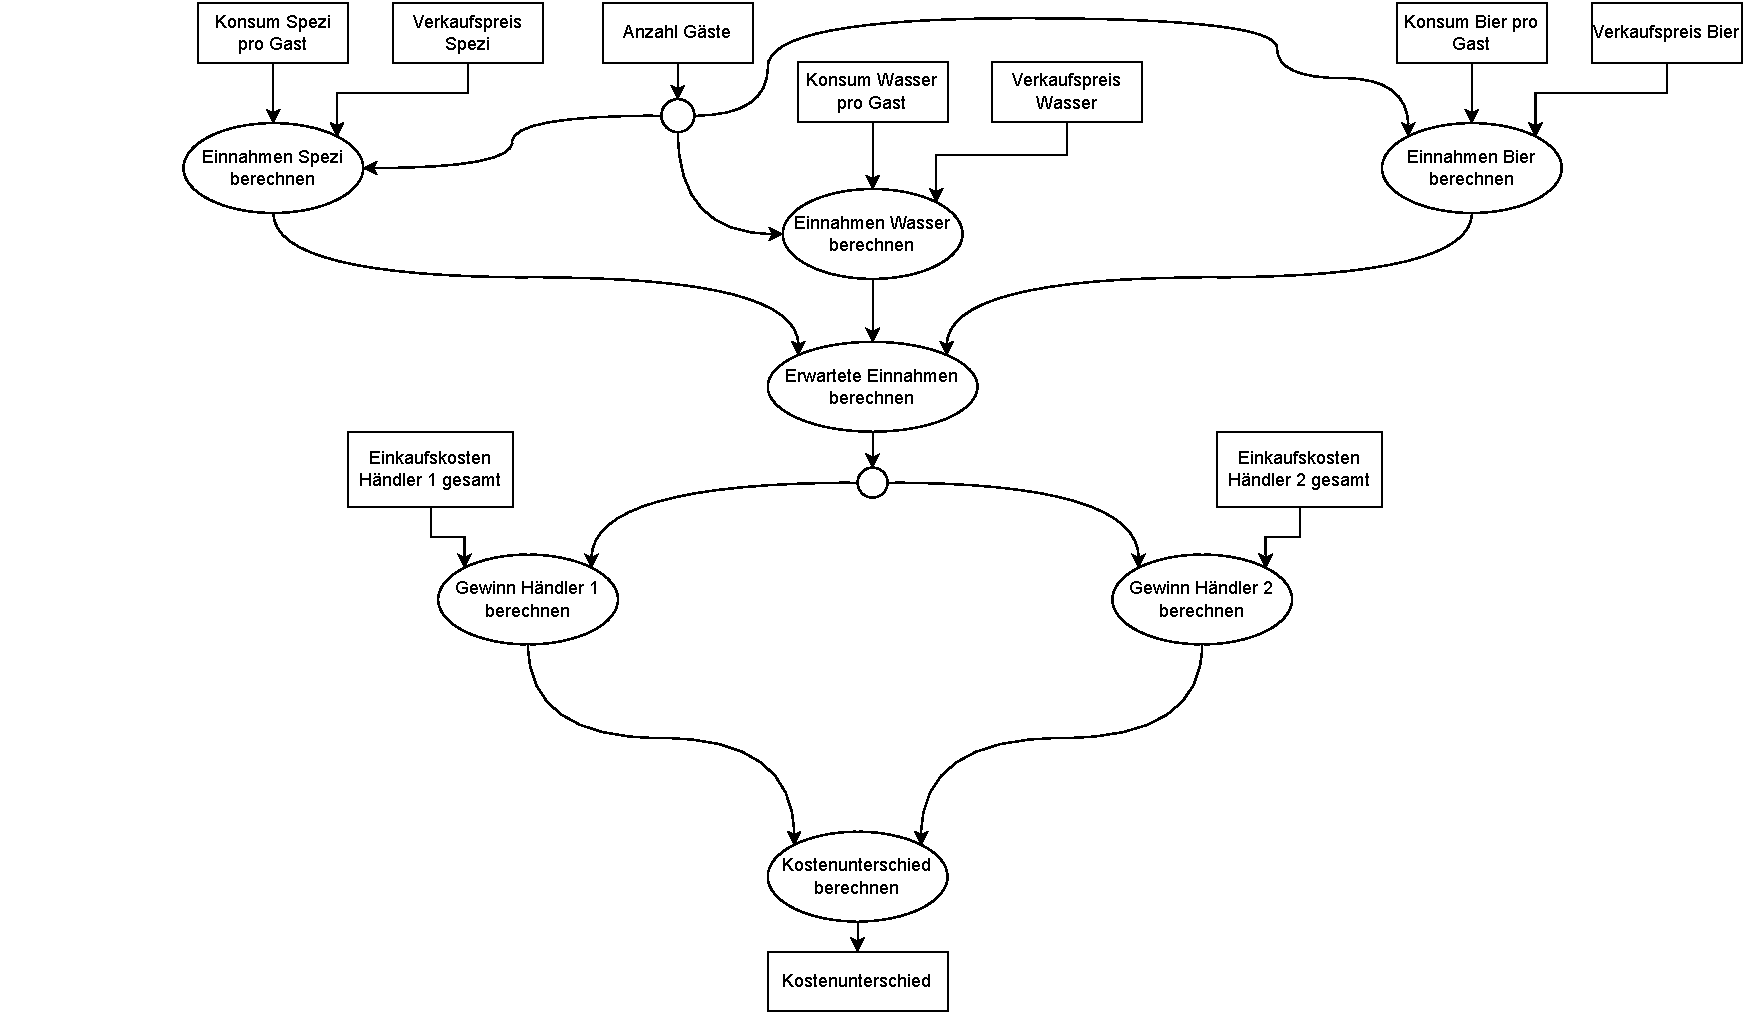
\includegraphics[height=\pageheight]{_Aufgaben/img/A06_Lsg_B04.pdf}
        }
    \else
        \UnterAufgabe{Gruppe B vereinfacht}{
            \Loesung{Gruppe B vereinfacht}
            
            \LoesungKaro{
                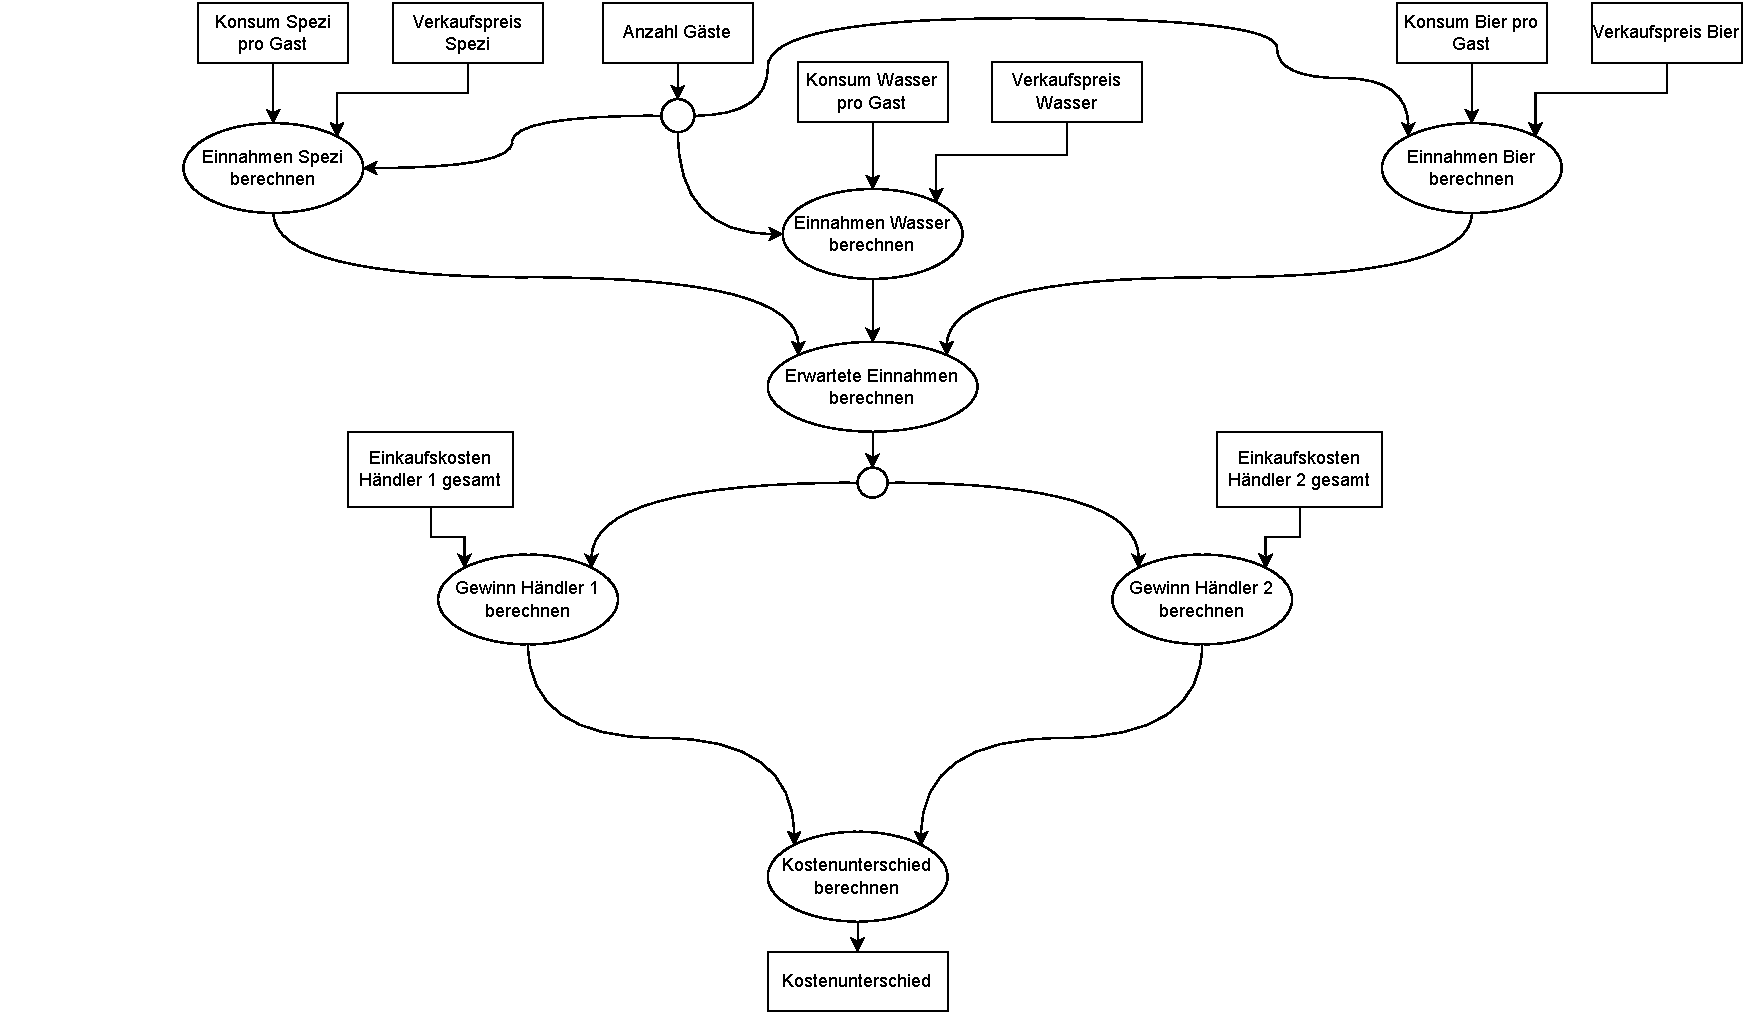
\includegraphics[width=\textwidth]{_Aufgaben/img/A06_Lsg_B04.pdf}
            }{51}
        }
    \fi